\documentclass[12pt,a4paper]{article}
\usepackage{amsmath}
\usepackage{amsfonts}
\usepackage{amssymb}
\usepackage{graphicx}
\usepackage{secdot}
\usepackage{multirow}
\usepackage[left=2cm,right=2cm,top=2cm,bottom=2cm]{geometry}

\title{{Experiment - 4\\ \textbf{Calibration of wind tunnel and verification of Bernoulli's equation}}}
\author{Arka Pramanick, AE21B007\\ Department of Aerospace Engineering\\ IIT Madras\\[3ex] Instructor:\\ \large Professor Dr. R. Sriram}

\date{5 March, 2023}


\begin{document}
\maketitle

\hline

\section{Aim :}
\begin{itemize}
    \item Calibration of wind Tunnel.
    \item Verification of Bernoulli's equaqtion.
\end{itemize}


\section{Apparatus :}
Required apparatus for performing this experiment are:
\begin{itemize}
    \item Manometer
    \item C15-10 Armfield tunnel
    \item Pitot-static Probe
\end{itemize}

\begin{figure}[!ht]
	\begin{center}
		\framebox{
			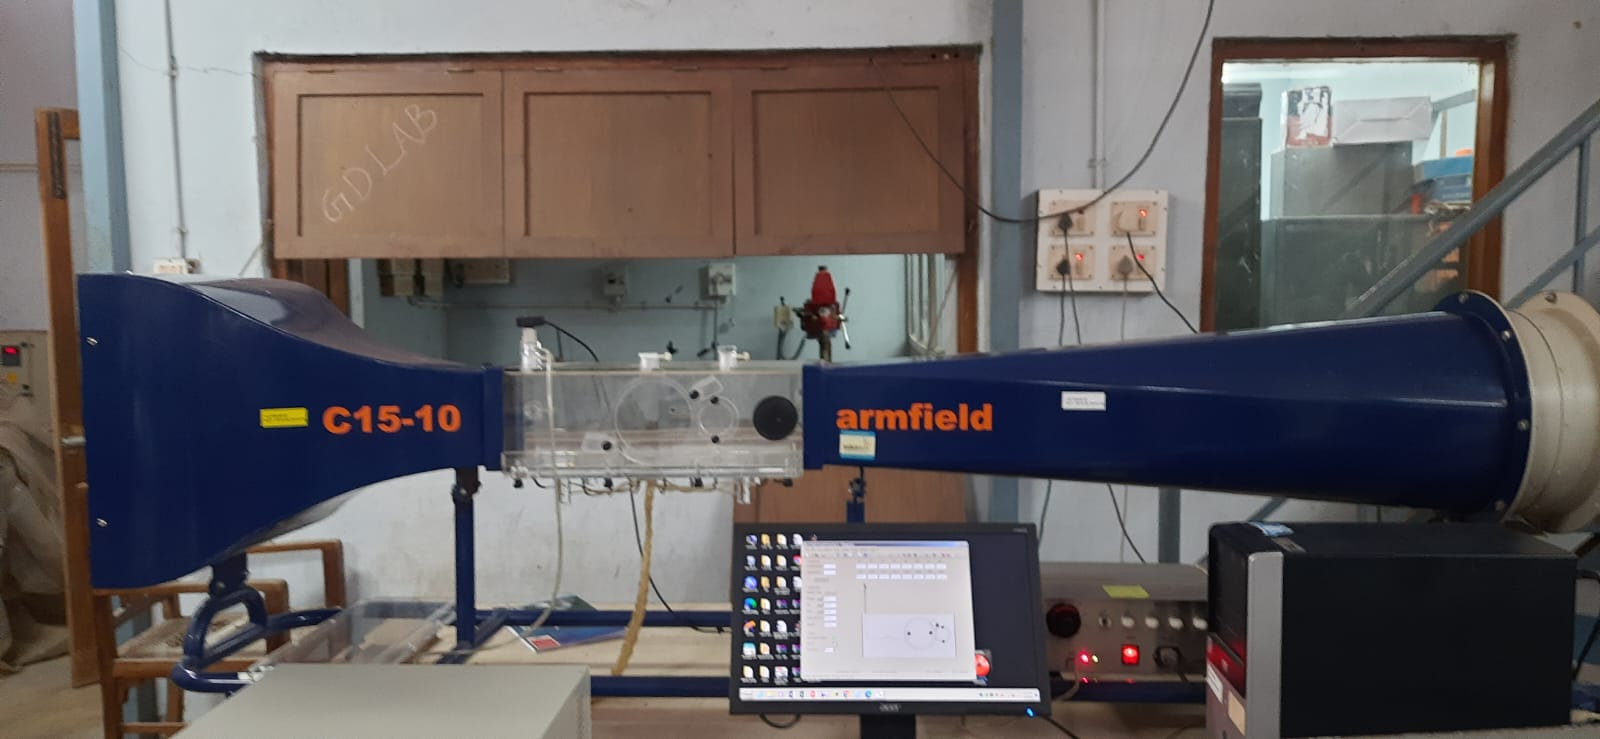
\includegraphics[scale=0.2]{wind tunnel.jpg}
		}
	\end{center}
	\caption{C15-10 Armfield}
\end{figure}


\newpage
\section{Theory :}

Bernoulli's Principle is basically the form of energy conservation.Bernoulli's equation has different forms and is used based on type of flow.Generally simplest form of the principle is applicable for both compressible flow and incompressible flow for most of the fluids at low Mach number only and more complicated form used for flows with higher Mach numbers.Bernoulli's equation states that :
\begin{equation}
    P_t = P_s + \frac{\rho v^{2}}{2}
\end{equation}
$P_t$ = Total Pressure/Stagnation Pressure;\\
$P_s$ = Static Pressure;\\ \vspace{2mm}
$\Delta P = P_t - P_s = \frac{\rho V^{2}}{2}$ = Dynamic Pressure\\
$\rho$ = Density of Air.
From eqn(1) : 
\begin{equation}
    \frac{\rho V^{2}}{2} = (P_t - P_s)
\end{equation}
\begin{center}
    $V^{2} = \frac{2(P_t - P_S)}{\rho}$ 
\end{center}
\begin{center}
    $V = \sqrt{\frac{2(P_t - P_S)}{\rho}} = \sqrt{\frac{2 (\Delta P)}{\rho}}$
\end{center}
   




\section{Procedure :}
\begin{enumerate}
    \item In wind tunnel test section is set.
    \item Pitot-static probe is connected to manometer.
    \item Fan speed is fixed.
    \item Required readings are taken.
\end{enumerate}






\section{Observation :}



\subsection{Experimental Data : } 

Ambient Temperature = 30$^{\circ}$ = 303 K\\
Ambient Pressure = 1018mBar = 101.8 KPa\\
Gas const.(R) = 287 J/Kg K






\subsection{Comparison of Theoretical Pressure and Experimental Pressure at different tapping point of Tunnel}


\begin{table}[ht]
\centering
\caption{\textbf{Pressure variation at different distance of Pipe and corresponding flow velocity}}
\vspace{2mm}
\begin{flushleft}
\begin{tabular}{|c|c|c|c|c|} 
 \hline
Tapping Point & Area(mm^{2}) & Velocity at port(m/s) & Theoretical Pressure(Pa) & Experimental Pressure(Pa) \\ [0.1ex] 
 \hline
$P_1$ & 22350 & 10  &  60.53 & 47.09 \\ 
 \hline
$P_2$ & 19860 & 11.25 & 76.08 & 57.88  \\
 \hline
$P_3$ & 17370 & 12.87 & 98.95 & 73.58  \\
 \hline
$P_4$ & 15000 & 14.9 & 131.94 & 99.08  \\
 \hline
$P_5$ & 15000 & 14.9 & 131.94 & 106.93 \\ 
 \hline
$P_6$ & 15000 & 14.9 & 131.94 & 110.85 \\ 
 \hline
$P_7$ & 16395 & 13.63 & 110.74 & 98.1\\
 \hline
$P_8$ & 17902.5 & 12.48 & 93.16 & 89.27\\
 \hline
$P_9$ & 19410 & 11.51 & 79.54 & 77.50 \\ 
 \hline 
$P_{10}$ & 20910 & 10.69 & 68.89 & 71.61 \\ 
 \hline 
$P_{11}$ & 22410 & 9.97 & 60.18 & 62.78 \\ 
 \hline
 
 
\end{tabular}
\end{flushleft}
\end{table}




\begin{figure}[!ht]
	\begin{center}
		\framebox{
			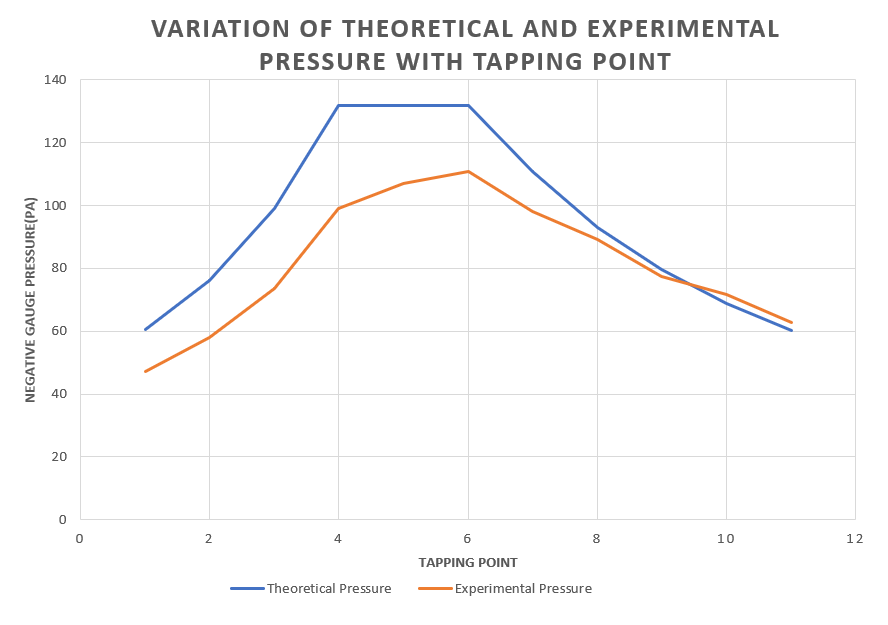
\includegraphics[scale=0.7]{pressure variation.png}
		}
	\end{center}
	\caption{Theoretical and Experimental Pressure variation with tapping point}
\end{figure}

\newpage

\subsection{Pressure and Velocity at 3 parts of wind tunnel :}

\begin{itemize}
    \item \textbf{Central Line :}\\
    Dynamic Pressure($\Delta P$) = 116 Pa \\
    Static Pressure($P_s$) = -118 Pa (Gauge Pressure) \\
    Stagnation Pressure($P_t$) =$P_t$+$P_s$ = -2 Pa (Gauge Pressure)\\
    Therefore, Velocity of flow = $\sqrt{\frac{2 (\Delta P)}{\rho}} = 14.08 $ m/s
    
    \item \textbf{35 mm Down :}\\
    Dynamic Pressure($\Delta P$) = 116 Pa \\
    Static Pressure($P_s$) = -118 Pa (Gauge Pressure) \\
    Stagnation Pressure($P_t$) =$P_t$+$P_s$ = -2 Pa (Gauge Pressure)\\
    Therefore, Velocity of flow = $\sqrt{\frac{2 (\Delta P)}{\rho}} = 14.08$ m/s
    \item \textbf{35 mm Above :}\\
    Dynamic Pressure($\Delta P$) = 108 Pa \\
    Static Pressure($P_s$) = -110 Pa (Gauge Pressure) \\
    Stagnation Pressure($P_t$) =$P_t$+$P_s$ = -2 Pa (Gauge Pressure)\\
    Therefore, Velocity of flow = $\sqrt{\frac{2 (\Delta P)}{\rho}} = 13.58 $ m/s
    
\end{itemize}

Flow velocity is almost uniform at a particular section of the tunnel.













\section{Calculations :}

Density of Air flow $(\rho) = \frac{P}{RT} = \frac{101800}{287 \times 303} = 1.1706$ $Kg/m^{3}$
\subsection{Theoretical Pressure Calculation :}


From experimental geometry we know area of each tapping point.\\
Speed of Fan($V_1$) = 10 m/s \\
We know,\\
$A_1$ = 22350 $mm^{2}$  , $V_1$ = 10 m/s , $A_2$ = 19860 $mm^{2}$ \\

\textbf{For tapping point $P_2$ :} \\
Using mass conservation principle : \\
$V_2 = \frac{A_1 V_1}{A_2} = 11.25 m/s $ \\
From Bernoulli's equation : \\
Dynamic Pressure $(\Delta P) = \frac{\rho v^{2}}{2} = 58.53 Pa$\\
Stagnation Pressure ($P_t$) = -2 Pa \\
Therefore, Static Pressure($P_s$) = -60.53 Pa (gauge) \\

Thus velocity is calculated at each tapping point and hence static pressure is calculated.


\subsection{Experimental Pressure Calculation :}
\textbf{For tapping point $P_2$ :}\\
Pressure at $P_2$ = -5.9 mm of Water\\
Static pressure = $ -5.9 \times 10^{-3} \times 10^{3} \times 9.81 = -57.88 Pa$(gauge)









\section{Sources of Error:}
\begin{itemize}
    \item Error due to instrumental defect.
    \item Error may occur in taking readings before flow becomes steady.
    \item Error due to environmental effect like temperature,pressure change.
\end{itemize}



\section{Conclusion :}
\begin{itemize}
    \item Experimental pressure variation across the tunnel(at different tapping point) is almost same with the tend of Theoretical Pressure variation. 
    \item Uniformity of flow is maintained throughout the wind tunnel.
    \item Bernoulli's equation is verified. 
\end{itemize}







\end{document}